\documentclass{article}
\usepackage[a4paper, top=3cm, bottom=2.5cm, left=2.5cm, right=2.5cm]{geometry} % Ajuste de márgenes
\usepackage[spanish]{babel}
\usepackage[utf8]{inputenc}
\usepackage{tikz}
\usepackage{titling}
\usepackage{graphicx}
\usepackage{fancyhdr}
\usepackage{amsmath}
\usepackage{amssymb}
\usepackage{multicol}
\usepackage{cancel}
\usepackage{pgfplots}
\usepackage{hyperref}
\usepackage{bookmark}
\pgfplotsset{compat=1.18}
\usepackage{titlesec} % Para personalizar títulos
\usepackage{tocloft}  % Para mejorar el índice
\usepackage{setspace} % Para controlar el espaciado

\usepackage{xcolor}
\usepackage{enumitem}

\definecolor{headerblue}{RGB}{50,90,140}
\definecolor{responsegray}{RGB}{80,80,80}



% Configuración de Fancyhdr para encabezados y pies de página
\pagestyle{fancy}
\fancyhf{}
\fancyhead[L]{
\includegraphics[width=2cm]{assets/logo-utp.png}}
\fancyhead[R]{\textbf{Diseño de Productos y Servicios}}

\fancyfoot[R]{\thepage} % Número de página alineado a la derecha

% Ajustes de espaciado entre párrafos y márgenes superiores
\setlength{\parskip}{1.5em}
\setlength{\parindent}{0pt}
\setlength{\headheight}{17.26935pt} % Altura del encabezado
\addtolength{\topmargin}{-2.26935pt} % Compensar el aumento de la altura del encabezado
\setlength{\textheight}{23cm}  % Ajusta el alto del texto

% Definición de comandos personalizados
\newcommand{\SubItem}[1]{
    {\setlength\itemindent{15pt} \item[-] #1}
}

% Título del documento con mejor control de espaciado
\title{
  
\includegraphics[width=5cm]{./assets/logo-utp.png} \\
  \vspace{1cm}
  \textbf{Universidad Tecnológica del Perú} \\
  \vspace{2cm}
  \textbf{Perfil de usuario, protopersona y segmentación de mercado} \\
  \vspace{1cm}
  \large \textbf{Para el curso de Diseño de Productos y Servicios.}
}
\author{
  \textbf{Luis Huatay Salcedo.} \\
  \textbf{Garcia Chumpitaz Cindel Roxell.} \\
  \textbf{Díaz Benítez, Fernando Raúl.} \\
  \textbf{Quispe Fernandez, Bryan Alexander.}
}


\begin{document}
\maketitle
\begin{center}
  Sección 44698
\end{center}
\thispagestyle{empty}
\begin{center}
  Mg. Marcos Teodoro Yerren Huima  
\end{center}
\restoregeometry

% \newpage

% \begin{center}
%   \textbf{\Large Índice}
% \end{center}
% \vspace{0.5cm} % Espacio entre título y contenido

% \begin{spacing}{1.15} % Espaciado personalizado para mayor legibilidad
%   \noindent
%   \begin{enumerate}
%     \item Introducción
%   %   \item Problemática
%   %   \item Objetivo general
%   %   \begin{enumerate}
%   %     \item Objetivos específicos
%   %   \end{enumerate}
%   %   \item Términos estadísticos
%   %   \item Recolección de información
%     \end{enumerate}
% \end{spacing}

\newpage
\section*{Creando un Perfil de Usuario y una Protopersona}

\begin{figure}[h!]
    \centering
    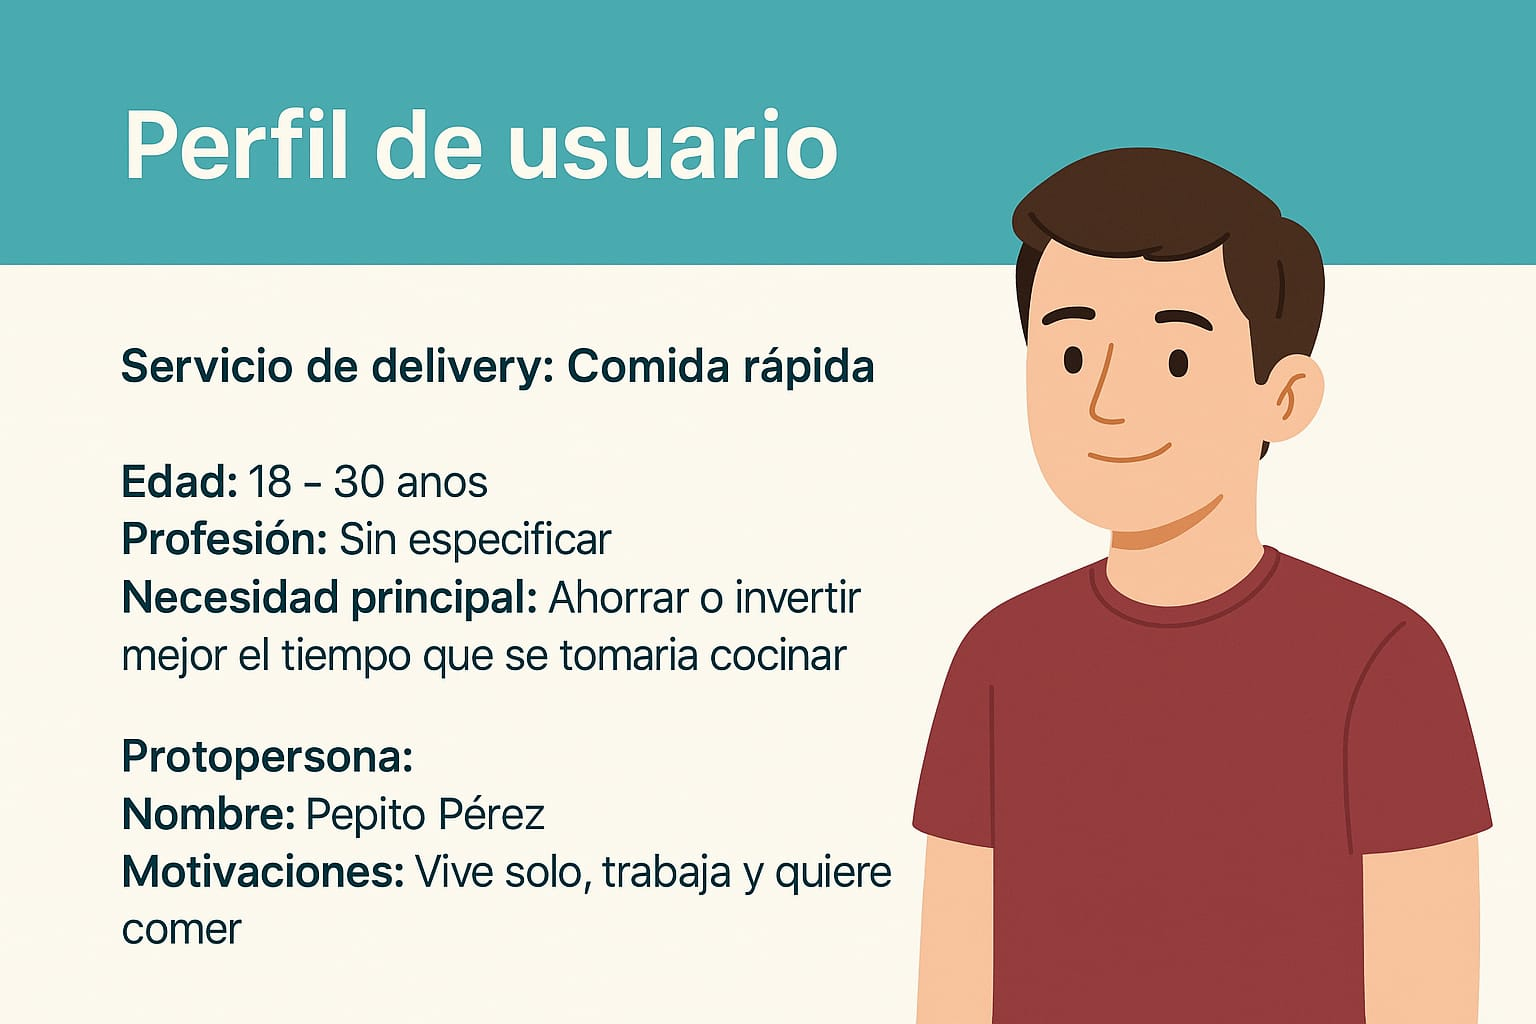
\includegraphics[width=0.7\textwidth]{assets/perfilDeUsuario.jpeg}
    \caption{Perfil de Usuario}
    \label{fig:segmentacion_mercado}
\end{figure}

\section*{Definiendo la Segmentación de Mercado}

\begin{figure}[h!]
    \centering
    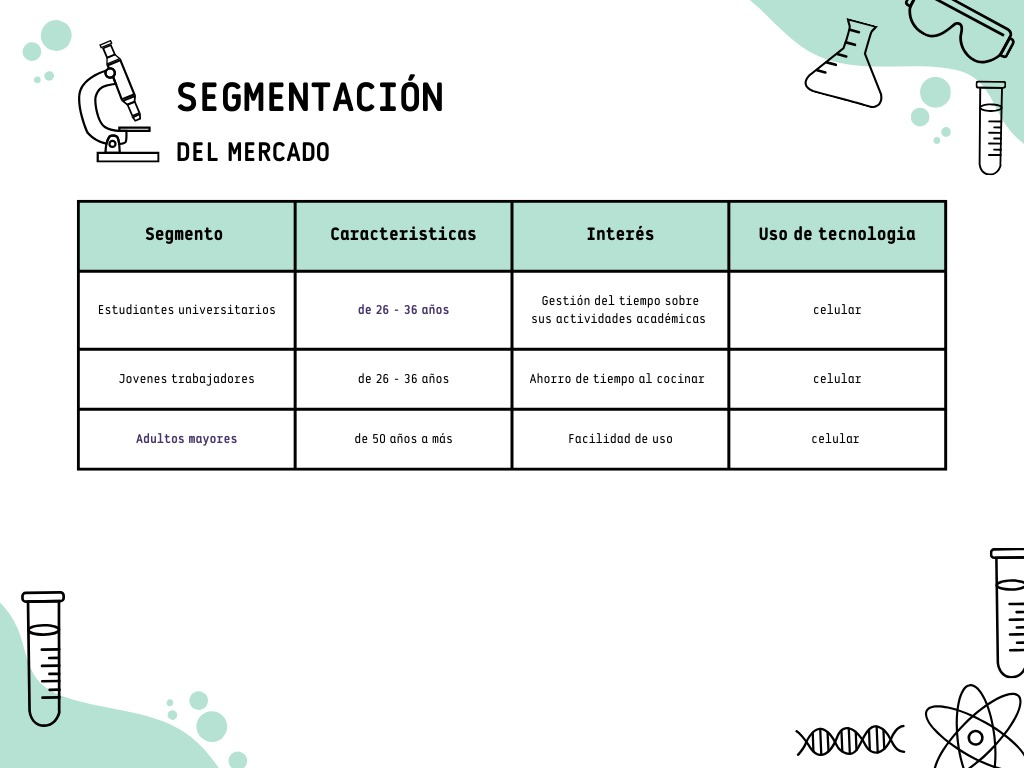
\includegraphics[width=0.8\textwidth]{assets/segmentaciion.jpeg}
    \caption{Segmentación de Mercado}
    \label{fig:perfil_usuario}
\end{figure}

\end{document}